% !TeX spellcheck = hu_HU
% !TeX encoding = UTF-8
\chapter{A Linda nyelv}\label{ch:linda}

%Történelmileg a Linda \acrfull{smp} környezetben való használatra lett kitalálva.
%Ez azt jelenti, hogy a programot futtató környezetben azonos processzorok vannak összekapcsolva egy közös memória tartományra, amelyet mindegyikük szabadon tud felhasználni.
%Ennek az architektúrának a lehetőségeit próbálja kiaknázni, és lehetőséget nyújtani a párhuzamosan futtatható programok készítésére, a direkt memóriamanipulációból származó nehézségek elkerülésével.

\section{A nyelv bemutatása}

A Linda nyelv elméleti modellje egy egyszerű de általános lehetőséget biztosít párhuzamos programok megvalósítására.
Ehhez a célhoz egyszerűségét két dologból nyeríti.
Egyik, hogy a Linda \index{Linda} csak egy \un koordinációs nyelv \cite{morrison_wiki_2004}, és nem egy teljes értékű programozási nyelv saját magában.
Így nem még egy megtanulandó új nyelv, ami külön parallel programok készítését teszi lehetővé, hanem pár egyszerű művelet, amelyeket egy $h$ gazdanyelvbe illesztve változtatja azt egy párhuzamos $h$-Linda programozási nyelvvé \cite{ahuja_linda_1986}.
Ezen megközelítés ereje abban rejlik, hogy a fejlesztés nagy része ismert eszközökkel, megszokott környezetben történhet.
Hasonlóan látható a sikeressége is, hiszen eredetileg a készítők a C (\textit{C-Linda}) és Fortran (\textit{Fortran-Linda}) programozási nyelvek kiterjesztéseként hozták létre \cite{ahuja_linda_1986}, azonban az évek során sok másik nyelvhez készültek külső fejlesztőktől különböző megvalósítások.
Ezek között találhatóak több esetben a HPC környezetben klasszikusan előforduló nyelveken kívül, elsősorban nagyvállalati kontextusban használt nyelvek is; ilyenek többek közt a Java \cite{sun_microsystems_javaspaces_2011, lehman_hitting_2001}, de még szkript nyelvekhez, mint például a Ruby, is készültek implementációk \cite[Part 3 -- Rinda]{seki_druby_nodate}.

A másik kulcsa az egyszerűségnek, hogy az előzőekben leírt gazdanyelv kiegészítéséhez pusztán hat műveletet vagy szabad függvényt ({\selectlanguage{english}free function}) használ fel.
Ezek mindegyike egy--egy egyszerű részfeladatot old meg a párhuzamos működés megvalósítása érdekében: az összes processzel megosztott \un\nes{} tér (\textit{tuple--space}, innentől, az eredeti publikációt követve: \ts, \cite{ahuja_linda_1986}) állapotának olvasását vagy módosítását teszik lehetővé a programozó számára.
Ebben látszik egy osztott memóriás világbeli szemlélet: minden program és programrészlet, ugyan azt az \ts{}-t látja, és az ezen végzett módosításokon keresztül tudnak adatot átadni egymásnak.
Az osztott memória azonban sok extra munkát és odafigyelést igényel a programozó részéről.
Biztosítani kell, hogy az adott memóriaterületek írása/olvasása megfelelően legyen szinkronizálva a különböző számítási folyamatok közül: a gyakran előforduló problémák közül az egyik leggyakoribbak a versenyhelyzetek ({\selectlanguage{english}race condition}) és a pattok ({\selectlanguage{english}deadlock}), amelyek mindegyike a nem megfelelő zárolásból adódik a program \un{} kritikus szekcióiban.
A Linda által adott megoldás ezeket elfedi a programozó elől, hiszen a konkrét osztott erőforráson végezhető műveletek atomi utasításokként viselkednek, így a zárolás automatikusan megvalósul egy--egy adatelem felett.

Az előző bekezdésben a \ts, mint elsődleges eleme a Linda modelljének került bevezetésre. Ennek a pontos definiáláshoz azonban először szükség van pár alap építő elemre a Linda eszköztárban:

\begin{defn}[Linda típus]\label{def:linda-type}\index{Linda típus}
    Azon típusok halmaza, amelyeket a Linda rendszer képes megfelelően kezelni.
    Ennek feltétele, $\mathbb{T}$ típus esetén hogy:
    \begin{enumerate}
        \item Minden $\mathbb{T}$ típusú érték egyértelműen összehasonlítható egyenlőség operátor felhasználásával.
        \item Minden $\mathbb{T}$ típusú érték leképezhető bájtok olyan sorozatára, amelyből az eredeti érték egyértelműen visszaállítható.
        Máshogy megfogalmazva, $\mathbb{T}$ sorosítható.
    \end{enumerate}
\end{defn}

\begin{remark}
    \Aref{def:linda-type}.~definícióból látható, hogy a megadott halmaz mérete és konkrét elemei csupán a megvalósítástól függenek: a modell csak azokat a tulajdonságokat írja elő, amivel a keresést meg tudja valósítani a \ts--ben, és egy másik folyamatnak át tudja adni az adott értéket.
\end{remark}

\begin{defn}[Linda érték]\label{def:linda-value}\index{Linda érték}
    Olyan érték, amelyik típusa a Linda típusok halmazának eleme.
\end{defn}

\begin{defn}[Linda \nes]\label{def:linda-tuple}\index{Linda \nes}
    Tetszőleges ($n$) darab Linda értékből álló rendezett lista.
    Más szóval olyan ennes ($n$--es, tuple, $n$--tuple), amelyik minden eleme Linda érték.
\end{defn}

\begin{defn}[A Linda \ts]
    Minden futó programrészlet által Linda műveletekkel módosítható és lekérdezhető halmaz, amelynek elemei kizárólag Linda \nes{}ek.
\end{defn}

A Linda \ts{} definíciója említi, hogy módosítható és lekérdezhető halmazként viselkedik.
Azonban, a tárolt értékek mellett, a konkrét műveletek, amiket végrehajthatunk a halmazon, sem szabadon választhatóak: csak Linda műveletekkel lehetséges minden interakció a \ts--el.
Itt jelenik meg a szekció elején említett pár egyszerű művelet, amelyet a Linda beilleszt egy választott gazdanyelvbe, hogy azt párhuzamos programozási nyelvvé változtassa. Ezek definiciója látható \aref{def:linda-cmd}.~definícióban.

\begin{figure}[b!]
    \centering
%    \resizebox{\linewidth}{!}{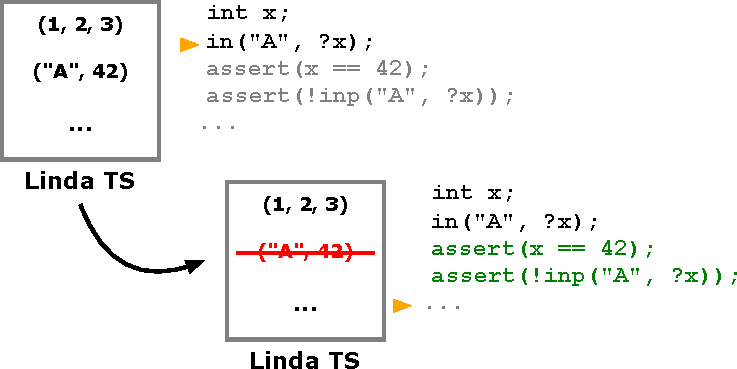
\includegraphics{figures/linda-in.pdf}}
    \caption{A Linda \lcmd{in} és \lcmd{inp} művelet}
    \label{fig:linda-in}
\end{figure}

\begin{defn}[Linda műveletek]\label{def:linda-cmd}\index{Linda művelet}
    A Linda modell által támogatott műveletek listája. Ezek a következőek:
    \begin{description}
        \item[\lcmd{in}($tuple\dots$)]
        \index{Linda parancs!in}
        Beolvassa és kitörli \ats{}--ből azt az \nes{} értéket, amelyik megfelel a paraméterként megadott \nes{}nek.
        Ha nem talál ilyen \nes{}t \ats{}--ben, akkor addig várakozik, ameddig egy megfelelő érték nem kerül beszúrásra.

        \item[\lcmd{inp}($tuple\dots$)]
        \index{Linda parancs!inp}
        A \lcmd{in} parancs nem blokkoló változata; beolvassa és kitörli azt az \nes{} értéket, amelyik megfelel a megadott \nes{} paraméternek.
        Ha nem talál ilyet, akkor hamis értékkel tér vissza, és nem hajt végre semmilyen műveletet.

        \item[\lcmd{rd}($tuple\dots$)]
        \index{Linda parancs!rd}
        Beolvassa, de nem törli ki \ats{}--ből azt az \nes{}t, amelyik megfelel a paraméter \nes{}nek.
        Ha nem talál ilyen \nes{}t \ats{}--ben, akkor addig várakozik, ameddig egy megfelelő érték nem kerül beszúrásra.

        \item[\lcmd{rdp}($tuple\dots$)]
        \index{Linda parancs!rdp}
        Az \lcmd{rd} parancs nem blokkoló változata; beolvassa, de nem törli ki \ats{}--ből azt az \nes{}t, amelyik megfelel a paraméter \nes{}nek.
        Ha nem talál ilyet, akkor hamis értékkel tér vissza, és nem hajt végre semmilyen műveletet.

        \item[\lcmd{out}($tuple\dots$)]
        \index{Linda parancs!out}
        Belerakja \ats{}--be a paraméter \nes{}t.
        Minden mező a parancsot kiadó folyamatban kerül kiértékelésre.

        \item[\lcmd{eval}($tuple^*\dots$)]
        \index{Linda parancs!eval}
        Belerakja \ats{}--be a paraméter \nes{}t.
        Egyes speciális függvényhívást tartalmazó mezők a paraméter \nes{}ben külön folyamatként kerülnek kiszámításra.
        Az így indított számítások lefutását nem várja meg az parancsot kiadó processz, hanem a fut tovább az eredeti kód.
    \end{description}
\end{defn}

Az műveletek megadásában található $tuple...$, egyes Linda értékekkel megadott Linda \nes{}, hozzá véve még \aref{subsec:qm-op}.~szekcióban ismertetett lehetőséget.
Az \lcmd{eval}-ban látható $tuple^*...$ paraméter értelmezésére a következőkben fog szó esni \aref{subsec:eval-fn}.~szekcióban.

Míg az \lcmd{out} működése egyszerű és egyértelmű, az \lcmd{in(p)} és \lcmd{rd(p)} függvényekhez tartoznak a megértést segítő \ref{fig:linda-in}.\ és \ref{fig:linda-rd}.~ábrák.
Ezeken a TS módosulása az \lcmd{in} esetében, és az általános egyszer mintaillesztés szerinti keresési viselkedés látható: az \lcmd{in} művelet utáni újbóli olvasás \lcmd{inp} segítségével már sikertelen olvasást eredményez, mert az \lcmd{in} azt kivette a TS--ből, amikor megtalálta.
Ugyan ez \lcmd{rd} esetén nem jelentkezik, ott bennmarad a TS--ben a megtalált ennes.

\begin{figure}[htb]
%    \resizebox{\linewidth}{!}{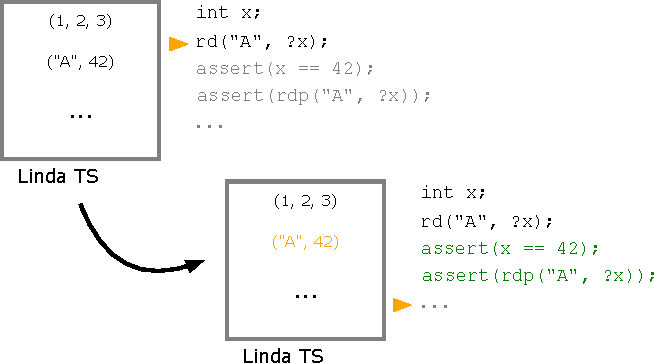
\includegraphics{figures/linda-rd.pdf}}
    \caption{A Linda \lcmd{rd} és \lcmd{rdp} művelet}
    \label{fig:linda-rd}
\end{figure}


%\begin{figure}[htb]
%    \resizebox{\linewidth}{!}{\includegraphics{figures/linda-out.pdf}}
%    \caption{A Linda \lcmd{out} művelet}
%    \label{fig:linda-out}
%\end{figure}

\subsection{A ?--operátor} \label{subsec:qm-op}

Ha csak az eddigiekben definiált műveletekkel rendelkezünk, akkor felmerül az a probléma, hogy csak azokat az \nes\ értékeket vagyunk képesek kivenni \ats{}--ből, amelyeket tudjuk, hogy benne vannak---vagy a program lefutása során bele fognak kerülni valamikor.
Esetlegesen még lekérdezhetjük, hogy egy adott \nes{} benne van-e \ats{}--ben, az \lcmd{inp} vagy \lcmd{rdp} függvények valamelyikével, de ennél többet nem tudunk tenni.

Ennek megoldására került bevezetésre a ?--operátor.
Egy változót felhasználva a ?--operátorral lehetséges általánosabb kereséseket végezni \ats{} tartalmán: a konkrét értékekként megadott mezők, mint keresési feltételek, és a keresett mezők típusa behatárolja, hogy melyik Linda \nes{}t találja meg a lekérdezés, majd a megfelelő változókba másolja a lekérdezett mezők értékeit. Erről látható egy szemléletes ábra \aref{fig:query}.~ábrán, illetve \aref{fig:linda-in}.\ és \aref{fig:linda-rd}.~ábrákon is látható a használata.
Az alapvető művelet az adatot tároló mezők kimásolása után történik meg, pl. az \lcmd{in} művelet esetén a törlés \ats{}--ből.

\begin{figure}[htb]
    \centerline{\resizebox{.75\linewidth}{!}{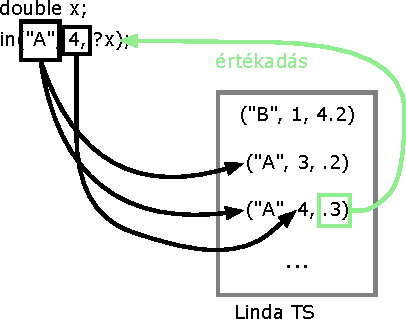
\includegraphics{figures/query.pdf}}}
    \caption{A paraméterezett keresés}
    \label{fig:query}
\end{figure}

\subsection{Az \lcmd{eval} függvény} \label{subsec:eval-fn}

Az \lcmd{eval} egy speciális függvény, miszerint a paramétereként megadott függvények, a $tuple^*...$ paraméterlistában nem helyileg kerülnek kiértékelésre, hanem egy új--de legalább egy már futó és különböző--folyamatban fognak lefutni, amelyből elérhető számukra a jelenlegi folyamathoz is tartozó Linda \ts{}.
Az így elindított részprogramok lefutását nem várja meg az indító kódrészlet, amint elindításra kerültek, folytatja futását.
Amikor minden függvény kiértékelésre került, az esetleges nem függvényként megadott konkrét Linda értékek és a lefutott függvények visszatérési értékei (amelyekről elvárt, hogy Linda értékek legyenek) listájából képzett Linda \nes{} beszúródik a Linda \ts{}--be, mintha az egyszerűen egy \lcmd{out} művelettel került volna bele.

Az \lcmd{eval} és a \lcmd{out} közötti különbséget szemlélteti \aref{fig:linda-eval}.~ábra.
Látható, hogy egy \lcmd{out} műveletet az azt kezdeményező függvény hajtja végre.
Egy \lcmd{eval} esetében azonban szükség van az egyes mezők másik folyamatok által számolt értékeire.
Így elsőként annak a visszatérését kapjuk meg, majd azzal képzünk egy \nes{}t.
Ami azonban a legfontosabb, hogy amíg az \lcmd{eval} hiányzó mezőire várunk, az eredeti függvény fut tovább.
Ez teszi lehetővé a párhuzamosítást, hiszen ahány párhuzamos példányt szeretnénk futtatni, annyit tudunk egy \lcmd{eval} segítségével indítani egy--egy adott függvényből.

\begin{figure}[htb]
    \resizebox{\linewidth}{!}{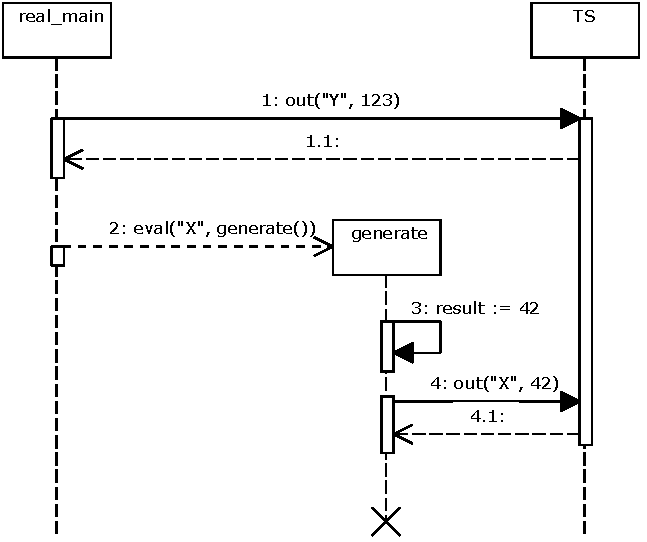
\includegraphics{figures/linda-eval.pdf}}
    \caption{A Linda \lcmd{eval} művelet}
    \label{fig:linda-eval}
\end{figure}

\section{A megvalósítás}

Ez a szekció tárgyalja a jelen dolgozathoz megvalósított Linda rendszer belső részleteit.
Leírja az általános architektúrától kezdve a fontosabb részleteket a rendszerről.
Emellett kitér azokra a dolgokra, amiket változtatni kellett az előzőekben leírt elméleti Linda nyelvtől, pusztán a gazdanyelv által nem támogatott lehetőségek miatt.

\subsection{A felhasznált eszközök}\label{subsec:tools}

Mivel a feladat fontos része, hogy hordozható és modern eszközök kerüljenek felhasználásra, így a megvalósítás C++-al, ezen belül is a 2020-ban kiadott szabványnak megfelelő verzióval történt (ISO/IEC 14882:2020).
Ezen Linda megvalósítás egy statikus könyvtárrá fordul, amely magában hordoz minden Lindához szükséges extra függőséget, használatához pusztán ezt a könyvtárat kell linkelni a programhoz.
A fordítás Clang ($17.0.3$) és MSVC ($19.40.33807$) fordítókkal működik és ezen fordítók zárójelekben megadott verzióikkal lett tesztelve.

A többszálúság megvalósítására a választott nyelv által biztosított szálkezelési primitívek kerültek felhasználásra, így ehhez nincs szükség külső könyvtárra.
A szálak egyszerű \texttt{std::thread} (és \texttt{std::jthread}) objektumokként vannak kezelve, amelyek a szabványos könyvtárban definiált szinkronizációs eszközöket használják fel az egymás közötti koordináció megvalósítására.
Ezek mellett pár helyen az \texttt{std::atomic<T>} sablon is felhasználásra került zárolás--mentes algoritmusok megvalósítására, pl.\ egy folyamat szintű monoton számláló így került implementálásra.

Fontos megjegyezni, hogy az egyik legelterjedtebb párhuzamosítási könyvtár, az OpenMP, miért nem lett választva.
A szál--párhuzamosított részei a programnak nagy részben \aref{subsec:ranks}.~szekcióban tárgyalt thread--pool megvalósítás részeként üzemelnek, ami mellett egy--egy segéd szál végez még érdemi munkát.
Ezek azonban sokáig futó szálak, amelyek gyakorlatilag csak a program legvégén lépnek ki.
Ilyen például a beérkező üzeneteket feldolgozó szál.
Ezt a struktúrát könnyebnek véltem a C++ beépített eszközeivel megvalósítani.

Emellett még előfordulhatnak párhuzamosítható ciklusok, amelyekre jól használható lenne az OpenMP.
Bár nem sok található meg a teljes kódbázisban, ezek nagy része is a sorosítási folyamat valamelyik lépése, amelyik valahogyan nem függ a többitől.
Ezek azonban kis számosságuk miatt nem véltek jelentős párhuzamosíthatósági kérdésnek, így a C++ által biztosított \texttt{std::execution::par\_unseq} direktívával ellátott szabványos algoritmusok is megfelelően működnek, jelentős kódmódosítás nélkül.
Ezen érvek miatt nem került felhasználásra az OpenMP.

A szálak mellett a processz szintű parallelizáció pedig az MPI könyvtárat használja fel.
Ezzel elérhető, hogy a Linda implementáció használható bármely olyan platformon, ahol létezik egy MPI megvalósítás.
Ez napjainkban az összes elterjedt és fontos platformra igaz.
A tesztelés MSMPI, OpenMPI és MPICH könyvtárakkal lett végezve, ilyen sorrendben Microsoft Windows, Fedora Linux és RedHat Enterprise Linux operációs rendszerek alatt.
Ezen opciók mellett is az MPI könyvtár elérhető a HPC környezetekben, akár különböző megvalósításokban (pl.\ Intel MPI), amin keresztül lehetségessé válik a Linda rendszer használata különböző szuperszámítógépre skálázott feladatokkal, kihasználva a biztosított számítási és párhuzamosítási kapacitást.
Manuálisan megvalósított folyamatindításokkal ez jelentősen nehezebben, vagy egyáltalán nem valósítható meg, és a különböző optimalizációkat is elveszítjük, amelyet az esetleges konkrét hardverhez tartozó MPI környezet biztosítana.

A Linda \ts{} elkészítéshez használt adatbázis a PostgreSQL.
Konkrétan a 17-es verzióval lett a működés tesztelve, de régebbi verziókkal is kompatibilis a kód egészen a 9.2--es verzióig: minden használt kliens oldali képesség már régóta létezik a PostgreSQL--ben.
Több okból esett erre az adatbázis-kezelőre a választás; ezek az alábbiak.
Fontos döntési pont volt, hogy egy megbízható, jó történelemmel rendelkező ACID kompatibilis adatbázist valósít meg, hiszen így a Linda \ts{} könnyedén tudja garantálni, hogy az atomi műveletek (tranzakciókba zárva) csak egészében futnak le, és izolálva vannak más folyamatok műveleteitől.
Emellett előnyben részesítettem a PostgreSQL--t, a nyílt forráskódja miatt, ami egy kifejezetten jól strukturált és dokumentált C kódbázis.
Ez jelentősen könnyebbé tette a kódhoz való hozzáillesztését, és a szerver oldali bővítmény fejlesztését.
Utolsó előnye pedig, hogy egy ORDBMS ({\selectlanguage{english}Object-Relational Database Management System}), azaz objektum-relációs adatbázis kezelő rendszer: lehetővé teszi, hogy saját, akár összetett típusokat lehessen definiálni, amelyeknek a tárolására alkalmas.
Ezek lehetnek egyszerű struktúrák, de teljesen saját típusokat is lehetséges megvalósítani saját konverziós függvények megadásával, sőt a nagyon különleges viselkedésű típusokra még az optimalizáló számára is lehetséges segédfüggvényeket definiálni a típus használatával kapcsolatban.
Arról, hogy ezeket a lehetőségeket hogy használja ki a megvalósítás, több szó esik
\aref{subsec:the-lts}.~szekcióban.

\subsection{Eltérések a modelltől}\label{subsec:diff-to-ideal}

A jelenlegi megvalósítás próbálkozik, hogy a lehető legközelebb maradjon a bemutatott elméleti Linda modellhez.
Azonban két helyen ezt a teljes illeszkedést nem sikerült tartani, a használt gazdanyelv rugalmatlanságából adódóan.

Az első a ?--operátor, ahogy \aref{subsec:qm-op}.~szekcióban be lett mutatva, sajnos nem megvalósítható C++ nyelven.
Mivel ez magában nem egy létező C++ operátor, amit túl lehetne terhelni, új operátorok felvételét pedig a nyelv nem támogatja.
A legközelebbi szintaktikával a \texttt{?:}, avagy a feltételes operátor, rendelkezik hiszen ez tartalmazza egyedül a kérdőjel karaktert, viszont ennek elválaszthatatlan párja a kettőspont.
Ugyanakkor, ha valahogyan még meg is lehetne oldani, valamiféle rafinált előfeldolgozási lépésekkel, hogy kettőspontok a kód megfelelő részeire bekerüljenek, akkor is szembesülnénk azzal megoldhatatlan problémával, hogy ezt az operátort nem lehet felüldefiniálni, amivel ez az egész irány zsákutcává változik.

Ezt megoldandó, egy saját megoldás bevezetésére van szükség: ez lett
az \texttt{ldb::ref}, amelyik egy mutatót vesz át arra a változóra, amelyiket a lekérdezésben szerepeltetni szeretnénk, és készít belőle egy olyan belső típust, amelyik alapján a lekérdezés végrehajtó tudja, hogy egyenlőség illesztéskor, ebbe a mutatóba bele kell írni az illeszkedő \nes{} megfelelő pozíciójú mezőjének értékét.
Az elnevezése a nyelv szabványos könyvtárában megtalálható \texttt{std::ref} függvényre utal.

A ?--operátor egyszerű, és alapvetően az eredetitől nem nagyon különböző, megoldással végződő nehézségeihez képest az \lcmd{eval} függvény egy komplexebb problémával szembesít.
A benne szereplő függvények szintaktikája teljesen megegyezik az egyszerű függvényhívás nyelvi szintaktikájával, és mégis egy teljesen más, inkompatibilis szemantikával rendelkezik.
Ennek megfelelően, valahogyan meg kell szakítani a függvényhívást az \lcmd{eval} paraméterlistájában, és átalakítani egy másik folyamatban kiértékelődő, de azonos tartalmú és jelentésű, függvényhívássá.

Ennek a helyzetnek az eredetihez leghűebb megoldásához a C++ makróihoz kell fordulni.
Ennek oka, hogy már a sablonok szintjén a függvényhívás, mint művelet,
nem állítható vissza egy függvénnyé, amit meghívnak, és egy híváshoz tartozó paraméterhalmazzá.
Sajnos, teljes azonosság még a makrók felhasználásával sem megoldható, mert az előzőekben említett függvény és paraméterlista kettest nem lehet előállítani egy tényleges függvényhívás szintaktikájából.
A sablonokkal ellentétben azonban, az előfeldolgozó képes arra, hogy, ha a függvényhívásnál a függvény is külön zárójellel van körbefogva (pl.\ \texttt{(fv)(1, 2)}), akkor ezt a konstrukciót a függvény nevét tartalmazó sztringre, a függvényre mutató mutatóra és a paraméterek listájára bontsa szét.

Ezekből az adatokból megkonstruálható egy globális {\selectlanguage{english}LUT}, amelyik az egyes függvények neveihez rendeli a függvénymutatókat.
Ha ezt a program futásának elején, statikus inicializálókkal valósítjuk meg, figyelve, hogy a globális statikus változók nem specifikált inicializálási sorrendje ne okozzon problémát, akkor a program bármely futó folyamata rendelkezik a számára helyes sztring--függvénymutató összerendelésekkel.

\begin{figure}[hbt!]
    \begin{subfigure}[h]{.4\linewidth}
        \begin{lstlisting}[numbers=left,language=C]
int x = 0;
out("params", 1, 2, 3);
eval("result", calc("params"));
in("result", ?x);
\end{lstlisting} % do not indent
        \caption{Az eredeti Linda}
    \end{subfigure}
    \hfill
    \begin{subfigure}[h]{.4\linewidth}
        \begin{lstlisting}[numbers=left,language=C]
int x = 0;
out("params", 1, 2, 3);
eval("result", (calc)("params"));
in("result", ldb::ref(&x));
\end{lstlisting} % do not indent
        \caption{A megvalósított Linda}
    \end{subfigure}
    \caption{A megvalósítás eltérései a modelltől}
    \label{lst:impl-diff}
\end{figure}

\subsection{Összesített architektúra}\label{subsec:lrt-arch}

A megvalósítás alapvetően egy MPI alapú párhuzamos rendszer.
Minden MPI rank, saját magába foglal egy végrehajtó egységet, amely a különböző Linda \lcmd{eval} által indított folyamatokat futtatja.
Emellett található egy külön folyamatban elhelyezkedő adatbázis rendszer, amelyik a \ts{} feladatát látja el.
Erről ad \aref{fig:linda-arch}.~ábra áttekintést, amelyen 3 rank közötti lehetséges kommunikációt szemléltet egy UML kommunikációs diagramot felhasználva.
A zölddel jelölt lifeline--ok az MPI kommunikátor részei, míg a kék szín a PostgreSQL processzben elhelyezkedő elemei a rendszernek.
Látható, hogy az \lcmd{eval} üzenetek a különböző rankok között direkt kerülnek eloszlásra, míg a primitív adat írás/olvasás műveletek egyenesen a postgres folyamat felé kerülnek irányításra.

\begin{figure}[htb]
%    \centerline{\resizebox{\linewidth}{!}{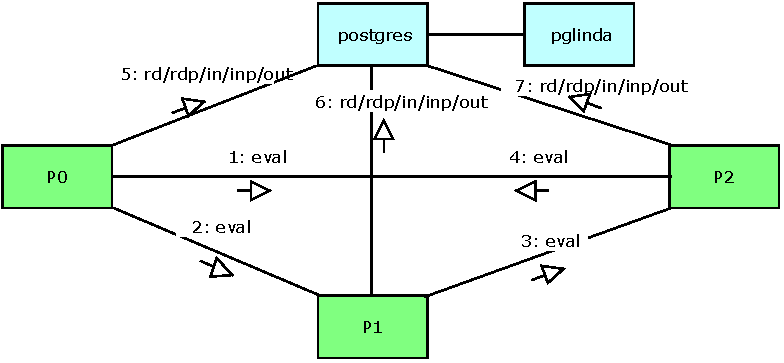
\includegraphics{figures/linda-arch.pdf}}}
    \caption{A Linda megvalósítás kommunikációs diagramja}
    \label{fig:linda-arch}
\end{figure}

\subsection{Egy rank feladata}\label{subsec:ranks}

Az előzőekben már olvasható módon, egy rank egy magában teljes számítási egységként viselkedik a globális számítás egy--egy részfeladatát végrehajtva.
Ehhez az architektúrához természetesen illeszkedik az MPI rankok egyenrangúsága, és hogy alapvetően minden rank ugyan azt a kódot kezdi el futtatni.
A Linda rendszer ezt jelentősen nem módosítja, az indított kód tényleg azonos a rankok között, egy apró különbséggel.

A $0.$ rank egy speciális feladatot hajt végre, ő szolgál a párhuzamos végrehajtás soros kezdőpontjaként.
Mivel a Linda program egy soros belépési pontnál indul, ezért az indításakor még nem fut semmi párhuzamosan, elméletben még az is lehetséges lenne az általános nyelvi elvek szerint, hogy nem is léteznek a folyamatok, amelyeken az \lcmd{eval} kiértékelések történnek.
Hogy ezt lehetővé tegye a megvalósítás, az MPI ellentétes viselkedése ellenére, a belépési pontot csak specifikusan a $0.$ rank futtatja, és a többi pedig várakozik arra, hogy az lefusson, amivel a teljes program végét jelzi.
Megjegyzendő, hogy ez nem zárja ki egyéb \lcmd{eval} parancsok végrehajtásától, a többszálú végrehajtásnak köszönhetően ezek egyszerre történhetnek egy rankon.

Ezt a speciális esetet leszámítva, minden rank azonos feladatot lát el, és azonos kódot futtat.
Egy szálon fut egy proaktor mintának megfelelő feladatot kezdeményező kódrészlet, amely a különböző beérkező MPI üzeneteket várja.
Annak beérkezésekor a megfelelő adatstruktúrává alakítja, és egy sorba helyezi el aszinkron végrehajtásra, amit egy thread--pool valósít meg.
Ebből egy--egy szál kiveszi a futtatandó feladatot, és elkezdi futtatni.
Az így futó kód felel meg egy--egy \lcmd{eval} függvény paraméterében meghívott függvény kiértékelésének, így ez is teljes értékű Linda kódként viselkedik: kezdeményezhet saját kommunikációt bármely Linda művelet segítségével, akár külön \lcmd{eval} parancsot is futtathat.
A lefutása végén a kiértékelt függvényhívásokkal, és a megfelelő egyszerű adat mezőkkel képzet ennes beírásara kerül a Linda \ts{}--be.

Azt, hogy kinek küldi el egy \lcmd{eval}--t elindító folyamat az üzenetet azt helyileg dönti el minden folyamat, amikor erre kerül a sor.
Ezzel a lokális döntéssel megspórolható egyéb kommunikáció, ami esetleg csak metaadatokat vinne a rankok között.
A választás algoritmusa jelenleg egyszerűen egy egyenletes eloszlású véletlen szám generátor, bár a kód ennek a választásáért felelős objektumot egy polimorf interfészen keresztül éri el, így könnyedén cserélhető egy szofisztikáltabb megoldásra, ha szükség volna rá.

A szimpla adatmódosító üzenetek azonban egyszerűbben kerülnek elküldésre, a teljes MPI infrastruktúrát valamilyen szinten megkerülve.
\Aref{subsubsec:serial}.~szekció szerinti sorosítás mezőnkénti végrehajtása után, a Linda \nes{}t egyszerűen a \mbox{PostgreSQL} szerver felé kerül elküldésre.
Itt azonban nem a teljes \nes{}t sorosítjuk, hanem mezőnként az értékeket.
Ennek a magyarázata, hogy az adatbázis kezelőnek egy SQL lekérdezést kell küldeni, amelyet az értelmezni és végrehajtani tud.
Ehhez az egyes mezőket egy paraméterezett lekérdezésben küldjük a szervernek, amelyik az egyes mezők értékét így egyesével fogja tudni felhasználni.
A szerveren ilyenkor lefutó folyamatokról \aref{subsec:the-lts}.~szekcióban található több információ.

\subsubsection{Sorosítás}\label{subsubsec:serial}

Az MPI környezet biztosít a fejlesztők számára eszközöket, amelyeket felhasználva saját típusok hozhatóak létre annak érdekében, hogy hatékonyabban lehessen nem primitív típusokat tartalmazó üzeneteket küldeni.
Az alap ötlet, hogy ezt felhasználva lehetséges megadni egy olyan leírást az MPI megvalósításnak, hogy az másolás nélkül ki tudja olvasni egy memóriapufferből az elküldendő adatokat.
Bár ez egy hatékonyságot jelentősen növelő és hasznos lehetőség, sajnos a jelenlegi célokra nem használható ki.
A Linda rendszer típusok szintjén mutatott dinamikusságát már nem tudja lekövetni: dinamikus hosszúságú tömbök (Linda \nes{}), amelyek egyesével lehetnek különböző típusúak (és ez által méretűek), ráadásul ezen mezők között is lehet olyan, amelyik dinamikus hosszúságú (sztring mező), de még rekurzívan másik \nes{}t tartalmazó is (függvényhívás jelölő).

Ennek eredményeképpen manuálisan kell megvalósítani a sorosítást.

Mivel az MPI egy C (és Fortran) keretrendszer, így ennek a megvalósítását pusztán egy bájt pufferbe való másolással tudjuk megoldani: első lépésben bejárjuk az \nes{}t, hogy kiderítsük, hogy az egyes mezők mekkora helyet foglalnak.
Ezt az információt felhasználva, hozzávéve egyes metaadatokat tartalmazó fejléceket az \nes{} és az egyes mezők szintjén, lefoglalunk ennyi memóriát, majd ismételt bejárással belemásoljuk az egyes értékeket és az ezekhez tartozó fejléceket.

A fejlécek tartalma igazán egyszerű: az \nes{} szintű metaadatok két értéket tartalmaznak, és egyszer szerepelnek a tartalom legelején.
Az első egy garantált $1$ értékű bájt, amely az üzenet tartalmát egyértelműsíti annak feldolgozása során.
Ezt követi egy 64--bites előjel nélkül értelmezendő szám, amely az \nes{} hosszát, azaz $n$ értékét tartalmazza.
Ezt követi pontosan $n$ darab mező leírása: egy bájt, amely a mező típusát tartalmazza, majd a mező típusától függő tartalom.
A típusonkénti leírás látható \aref{tbl:type-serial}.~táblázatban.
Ezeket nem követi semmi, azaz nincs az üzenet tartalmát lezáró része az üzenetnek; a fejlécekben megadott hosszúság metaadatokból következik, hogy mikor van vége az üzenetnek.

A lekérdezéseket megvalósító ?--operatárorral képzett speciális \nes{}ek is ezen rendszer szerint kerülnek sorosításra, az egyes hiányos mezők egy \un{}típus referencia mezőre kerülnek leképezésre; ez is megtalálható \aref{tbl:type-serial}.~táblázatban.

\def\lend{{\selectlanguage{english}little--endian}}
\def\bend{{\selectlanguage{english}big--endian}}

%\paragraph{A bájtsorrend problémája}
%A több bájton átívelő számértékek értelmezése processzor architektúra (vagy annak beállításának) függvénye, és emiatt egy több bájtos szám memóriaképe különbözhet két összekötött számítógépen, megnehezítve a kommunikációt.
%Ezt a problémát sok esetben automatikusan elintézi az MPI rendszer, ha magukat ezeket a számokat küldjük át; viszont a Linda saját sorosítási protokollt használ, és a sorosított bájtokat küldi, így manuálisan kell megvalósítania ennek a kezelését.
%Elterjedt megoldás \un{}hálózati bájtsorrendbe ({\selectlanguage{english}Network--endian}) kódolást használni kommunikáció során; ez a \bend.
%Ez azonban nem minden esetben éri meg, hiszen ha csak \lend{} konfigurációt használó processzorok vannak összekötve, akkor csak felesleges bájt cserélgetést okoz mind két oldalon.
%Mivel, \aref{sec:par-hw}.~szekcióban leírtaknak megfelelően, sok esetben x86-64 processzorok vannak felhasználva, mind HPC, mind asztali számítógép környezetben, amelyek szigorúan csak \lend{} konfigurációt használnak, így a Linda futtató környezet alapvetően képes mind két lehetőséget használni egy fordításkor megadható paraméter értéke szerint.
%Az fontos, hogy azonos fordítási beállítással legyen fordítva a két kommunikáló fél által használt könyvtár, mert alapértelmezetten a gazdagép által használt konfigurációt követi.
%Ezzel elérhető, hogy homogén rendszerek esetén a felhasznált architektúrának ideálisabb sorrendben lehetséges több bájtos számértéket küldeni akár \lend, akár \bend{} rendszereken.
%A PostgreSQL szerverrel való kommunikációnak mindenképpen \bend{} formában kell lennie, így az ilyen irányú kommunikációra ez a paragrafus nem vonatkozik.

\subsection{A Linda \ts}\label{subsec:the-lts}

Az egyik legfontosabb eleme a Linda rendszernek a Linda \ts{}.
Ezt a jelenlegi megvalósítás, az előzőekből már olvasható módon, a PostgreSQL adatbázis kezelőt felhasználva valósítja meg.

A PostgreSQL támogatja, hogy saját szerver oldali bővítményt valósítsunk meg, amelyben teljesen saját SQL--ből használható függvényeket lehet definiálni, sok különböző támogatott nyelvet felhasználva, például (alapból beépítve) PL/pgSQL, Perl, Tcl vagy Python.
Ezektől függetlenül egy C interfész is elérhető, amelyet az interpretált nyelvek is használnak; de lehetőségünk van nekünk is ezt használni.
Ezt a lehetőséget összeszinkronizálva a saját típusok megvalósításának biztosításával, amelyhez pusztán pár függvény definiálására van szükség, elérhető, hogy egy teljesen saját típust lehessen létrehozni egy szerver oldali bővítményben vagy C--ben, vagy bármely olyan nyelven, amelyik képes a C ABI--nak megfelelő szimbólumokat definiálni egy dinamikus könyvtárban (SO, DLL).
Mivel C++--al került megvalósításra a többi kódrészlet, így ez a bővítmény is C++--ban lett megírva, pár C nyelvű szimbólumot publikussá téve a könyvtárban.

A bővítmény magában elég egyszerű, minimális funkcionalitást valósít meg.
Összes feladata, ezzel szinkronban annyi, hogy a különböző rankok által küldött \nes{} objektumokat eltárolja, majd lehetővé tegye ezek között a keresést.
Ennek a célnak az eléréséhez két típust valósít meg a bővítmény.

Az egyik az \texttt{LV\_TYPE}, amely egy adott Linda típust azonosít.
A tényleges értéke egy 8--bites egész szám, amely egy kódot tárol, hogy melyik típusról van szó.
Elsőre limitálónak hangzik a pusztán 255 darab típus tárolásának lehetősége, de perspektívaként ebből a jelenlegi rendszer összesen 10 darabot használ, így van elég sok bővítési lehetőség.
Ráadásul, ha ez valamiért nem lenne elegendő, akkor a típus mérete növelhető azzal a feltétellel, hogy minden folyamat a frissített verziót várja el az adatbázistól.

A konkrét értékek a biztosított típusok esetén láthatóak \aref{tbl:type-serial}.~táblázat megfelelő oszlopában.
Ebben a típusban tárolt értékek konkrétan nem kerülnek tárolásra, csak a kereséses során vannak felhasználva, amikor olyan lekérdezés fut, amelyben egy adott típust adtunk csak meg, és nem egy konkrét Linda értéket.
Ennek ellenére semmi nem akadályozza, hogy ezt tárolná az adatbázis, pusztán nem volt rá szükség a tervezés és fejlesztés alatt.

A másik az \texttt{LV}, amelyik már magával a Linda típussal megfeleltethető az adatbázis szintjén, összegtípusként képes tárolni egy oszlopban az összes \ref{def:linda-type}.~definíció szerinti típust.
A jelen megvalósításban támogatottak \aref{tbl:type-serial}.~táblázatban látható típusok, azzal a megkötéssel, hogy a függvények tárolása nem az adatbázisban történik, így abban nem is került megvalósításra kezelésük.
(\ld \ref{subsec:lrt-arch}.~szekció az architektúráról, ami a függvények kezelését is taglalja.)
A ténylegesen tárolt rekord mezők tartalma is kiolvasható ugyanebből a táblázatból.
Amit fontos észrevenni, hogy a szám típusok (\texttt{int}, \texttt{unsigned}, \texttt{double}, stb.) tárolásánál pusztán a számot tárolja, és nem a sztring reprezentációját.

Ez a gondolatmenet egy alapvető hatékonysági kérdés.
Ha ezt nem tenné az adatbázis és karakterenként (feltételezve 8--bites karaktereket---egyes kódolásoknál (pl.~\hbox{UTF--16}) ez az arány még rosszabb) tároljuk el egy 64--bites szám értékét, akkor $64/8 = 8$ számjegyből álló szám esetén már több adatot tárolunk a sztring formátumban, mint számként.
Ami jelentősebb probléma azonban, hiszen a \hbox{diszk/memória} relatíve olcsó, hogy az adatokat össze is kell hasonlítani.
Két szám esetén egy megfelelő szómérettel rendelkező processzoron egy darab skalár utasítással megállapítható azoknak a relációja, de rövidebb szóméret esetén is csak 1--2 darab utasításról van szó, amelyek mindegyike egyszerű skalár művelet.
Szövegként tárolt megvalósítás esetén viszont minden karaktert egyesével kell összehasonlítani, vagy valamilyen SIMD vektorművelettel kell gyorsítani azt.
Ezek mindegyike jelentősen több munka, mint egy egyszerű \texttt{CMP} (vagy ekvivalens) utasítás lefuttatása, nem is számolva az esetleges manuális SIMD kód általában kimagaslóan ,,jó'' karbantarthatóságával.

Ezeknek a típusoknak a megvalósításához kellett megírni azokat a függvényeket, amelyek egy sztring reprezentációból a konkrét típusra konvertálják az értéket.
Így szükségszerű megadni egy sztring reprezentációt, ami egyértelműen meghatároz egy Linda értéket, és annak típusát.
Ez könnyen megvalósítható módon, egy kukac-szimbólummal (\texttt{@}) elválasztva a típus \aref{tbl:type-serial}.~táblázatbeli kódja hexadecimálisan majd a konkrét érték sztringként leírt értéke.
Pár példa érték látható \aref{lst:custom-sql-type}.~listázásban, annotálva az adott érték típusával.

\begin{lstlisting}[language=SQL, label=lst:custom-sql-type, caption={Saját típus támogatás PostgreSQL--ben}]
SELECT LV '0@123'    -- std::int16_t
     , LV '7@789'    -- std::uint64_t
     , LV 'A@1'      -- ldb::lv::type_ref, ami std::uint8_t-t tárol
     , LV '4@szöveg' -- std::string
\end{lstlisting}

Bár az előzőekben leírt függvénypár a minimum, amit biztosítani kell egy saját típus megvalósításához, egyéb függvények is megadhatóak, a különféle optimalizációk és extra lehetőségek elkészítéséhez.
Az egyik legegyértelműbb, a megfelelő bináris reprezentációból való konvertálás írás és olvasási műveleteknél.
Ehhez \aref{subsubsec:serial}.~szekcióban leírtak szerinti sorosítási eljárás került megvalósításra \mbox{PostgreSQL} oldalon is.

Ami még érdekes az adatbázisból a Linda megvalósításnak, az a kereshetőség biztosítása.
Ehhez az aritmetikai relációs műveleteket kell megvalósítani, és hozzárendelni az elvárt operátorokhoz ($<, <=, =, >=, >$).
A rendezettséget elsőként a típus alapján adhatjuk meg, és ha azok azonosak, akkor az érték szerinti összehasonlítás szerint.
Ezeket az operátorokat felhasználva pedig létrehozható egy olyan \un operátor osztály (operator class), amelyik egy B--fa alapú index megvalósítását teszi lehetővé egy LV típusú oszlop felett, gyorsítva a keresést.

% Kell-e ide a tömb típus?
% mmint a linda_data(first : LV, second : LV, stb : LV[]) séma érdekes-e

\begin{table}[htb]
    \begin{tabularx}{\linewidth}{|l|l||c|X|}
        \hline
        \textbf{C++ típusnév} & \textbf{Típus} & \textbf{Kód} & \textbf{Tartalom} \\
        \hline
        \texttt{std::int16\_t} & 16--bites előjeles egész & $0$ & A szám értéke \\\hline
        \texttt{std::uint16\_t} & 16--bites előjel nélküli egész & $1$ & A szám értéke \\\hline
        \texttt{std::int32\_t} & 32--bites előjeles egész & $2$ & A szám értéke \\\hline
        \texttt{std::uint32\_t} & 32--bites előjel nélküli egész & $3$ & A szám értéke \\\hline
        \texttt{std::string} & sztring & $4$ & A sztring hossza 64--bites előjel nélküli egész számként, majd a sztring bájtjai \\\hline
        \texttt{ldb::lv::fn\_call} & függvény hívás & $5$ & A sztringben leírtak szerint kódoltan a függvény neve, majd a rekurzívan \nes{}ként kódolva a paraméterei \\\hline
        \texttt{std::int64\_t} & 64--bites előjeles egész & $6$ & A szám értéke \\\hline
        \texttt{std::uint64\_t} & 64--bites előjel nélküli egész & $7$ & A szám értéke \\\hline
        \texttt{single} & egyszeres lebegőpontos szám & $8$ & A szám értéke \\\hline
        \texttt{double} & kétszeres lebegőpontos szám & $9$ & A szám értéke \\\hline
        \texttt{ldb::lv::type\_ref} & típus referencia & $A$ & A hivatkozott típus kódja 8--biten \\\hline
    \end{tabularx}
    \caption{A típusok sorosítási értékei}
    \label{tbl:type-serial}
\end{table}

\subsubsection{Keresés}

Keresést az adatbázisban kellett megvalósítani, különben túl sok adatot kellene a kliensek és az adatbázis között mozgatni, hogy hatékony maradhasson a megvalósítás.
Ez általános egy adatbázis használó alkalmazás esetében.
A Linda modell keresési logikája azonban két csoportra oszlik: amikor a teljes \nes{} tartalmát ismerjük, és azt keressük az adatbázisban; illetve amikor vannak olyan mezők, amelyek csak egy típust írnak elő.

Előbbit egyszerű megvalósítani, lényegében egy szimpla adatbázis lekérdezéssé alakítandó a keresett \nes{} úgy, hogy az adott indexű Linda érték illeszkedését nézzük az azonos indexű oszloppal a relációban.
Amire figyelni kell, hogy az egy \nes{} keresésénél a reláció $n + 1$. mezejét ellenőrizni kell, hogy SQL \texttt{NULL}, különben a keresetnél hosszabb, de azonos prefixű \nes{} értékeket is kiolvasnánk.

A második típusú keresés azonban jelentősen komplikáltabb, hiszen maga a keresés egy olyan dologra (a típusra) hivatkozik, amelyik csak fordítási időben létezik, egy másik program forráskódjában: a típust a Linda kód tartalmazza, de magát a keresést a PostgreSQL szerverének kell végrehajtania.
Ennek a problémának megoldására került bevezetésre az előzőekben már ismertetett \texttt{LV\_TYPE} SQL típus.
Mivel ez képes egy típus mivoltát ábrázolni, így pontosan megfelel olyan adatként szolgálni, ami alapján lehetséges típus alapú lekérdezéseket megvalósítani.
Ehhez a PostgreSQL függvény (és operátor) túlterhelési lehetőségét lehet kihasználni, amivel elérhető az, hogy \texttt{LV~$\Theta$~LV} műveletek mellett, az \texttt{LV~$\Theta$~LV\_TYPE} műveletek is létezzenek.
(Plusz kommutatív párok.)
Ha pedig már léteznek a megfelelő függvények és operátorok, akkor könnyen specifikálható a működésük úgy, hogy a típussal való összehasonlítás esetén az adott műveletet csak az érték típusán és a kapott típuson hajtjuk végre: ez pont egyezik az elvárt keresési feltételünkkel, és így beteljesedik az \nes{}ek keresése.

\subsubsection{Hatékony várakozás}

Egyes esetekben a Linda modell szerint várakozni kell, amíg valamilyen érték nem kerül be a \ts--be.
Ilyen esetek az \lcmd{in} és \lcmd{rd} műveletek, ha a keresett értékeket nem találja meg elsőre a \ts--ben.
Erre két megoldást lehet adni: adott időközönként újra lefuttatjuk a lekérdezést, majd annak eredménye alapján megyünk tovább, vagy ismételten újra keresünk.
Tehát aktívan várakozunk, és aktívan polloljuk az adatbázist.
Ez nyilván egy kifogásolható megoldás, hiszen nagyon sok fölösleges keresést generál az adatbázis számára.
Emellett még akkor is újra és újra elküldi ugyan azt a sikeresen lefutott, de eredményt nem adó lekérdezést, ha közben semmi változtatás nem történt a \ts--ben, így garantálhatóan nem fog sikerülni.

Általános esetben nem lehet azonban ennél jelentősen mást csinálni, esetleg a várakozások idejét finomítani vagy egyéb felületes optimalizációkat eszközölni.
Összességében a tényleges megoldás a pollolást problémájára, hogy valamilyen várakozást építünk a programba, amelyik addig passzívan várakoztatja a kérdező folyamatot, amíg valamilyen feltétel nem teljesül, ami javítja (vagy garantálja) a lekérdezés sikerességét.

Ennek az értesítésnek jelenleg az adatbázis oldaláról kell most származnia, hiszen ott történik meg az a módosítás, amelyik kiválthatja a kliens reakcióját.
Erre a feladatra a tökéletes megoldás ismételten egy PostgreSQL által nyújtott sajátos funkcionalitás: a \texttt{LISTEN} és \texttt{NOTIFY} SQL parancsok.
Ezek lehetővé teszik az adatbázis szerverhez kapcsolódott, és a hallgatózást elindító (\texttt{LISTEN}) klienseknek, hogy aszinkron értesítéseket kapjanak az adatbázistól, amikor bármelyik futó tranzakció kiadja a \texttt{NOTIFY} utasítást.
Ehhez lehetséges társítani egy rövid szöveges üzenetet is, amelyet a hallgatózó kliensek megkapnak.
Kihasználva ezt a lehetőséget, a beszúrt \nes{} érték elemeinek típusát azonosító számokat küldi el a szerver, amivel lehetővé teszi, hogy a klienseknek csak akkor kelljen újra elindítani a konkrét lekérdezést, ha a mezők típusai egyeznek, ezzel is minimalizálva a biztosan sikertelen lekérdezések futtatását, és könnyítve az adatbázis dolgát.
















